\chapter{简单机械：杠杆、滑轮、斜面}\label{ch:g5:simple-machines}

没有发动机，也没有电——但只用几根木梁、几条绳子和几个斜坡，
古代的建造者就能吊起整队牛都拖不动的石块。
他们的工具箱里装着\emph{\omterm{def:g5:simple-machines:machine}{简单机械}}：
这些发明没有发动机，却能把轻柔的拉力
变成强大的力量。你已经认识了第一种，现在来认识这个家族吧。

\section{省力工具家族}

\begin{definition}[简单机械]\label{def:g5:simple-machines:machine}
称\emph{简单机械}\index{简单机械}为一种没有
电动机、能按我们的需要改变力的装置：使力变大，
或改变力的方向，或两者兼有。经典的例子有你已熟悉的\emph{\omterm{def:g3:levers-and-scales:lever}{杠杆}}，
跷跷板和撬棍上的就是它；还有\emph{\omterm{def:g5:simple-machines:pulley}{滑轮}}，以及
\emph{\omterm{def:g5:simple-machines:ramp}{斜面}}——就是那个朴素的斜坡。
\end{definition}

\begin{example}[再看杠杆]\label{ex:g5:simple-machines:lever}
\omterm{def:g3:levers-and-scales:lever}{杠杆}的规律你已经知道：硬币数乘以刻度数——你的小力
离\omterm{def:g3:levers-and-scales:lever}{支点}远，就能胜过靠近\omterm{def:g3:levers-and-scales:lever}{支点}的大重物。注意还有一件事：
你握住的撬棍一端会向下划过很长的距离，
而石头只升高一点点。请把这个发现记在心里，
它很快就会变成一条规律。
\end{example}

\section{滑轮}

\begin{definition}[滑轮]\label{def:g5:simple-machines:pulley}
\emph{滑轮}\index{滑轮}是一个带有绳槽的轮子。
挂在横梁上的\emph{定滑轮}只改变拉力的
方向：向下拉，重物就向上升。一个\emph{动滑轮}
套在绳子上，重物挂在它下面：此时重物悬挂于
\emph{两}股绳子上，每股绳子只承担
一半的重量。
\end{definition}

\begin{omfigure}
\begin{tikzpicture}[scale=0.8]
  \draw[thick] (0.2,4.4) -- (2.8,4.4);
  \draw[thick] (1.5,4.4) circle (0.42);
  \draw[thick] (1.08,4.4) -- (1.08,1.6);
  \draw[thick] (1.92,4.4) -- (1.92,2.8);
  \draw[thick, fill=omMeth, fill opacity=0.4]
    (0.68,0.8) rectangle (1.48,1.6);
  \node[font=\footnotesize] at (1.08,1.2) {重物};
  \draw[-Stealth, very thick, omThm] (1.92,2.8) -- (1.92,1.9);
  \node[right, font=\small] at (2.1,2.3) {全力向下拉};
  \node[below, font=\small] at (1.5,0.3) {定滑轮：改变方向};
  \begin{scope}[xshift=6.6cm]
    \draw[thick] (0.2,4.4) -- (3.6,4.4);
    \draw[thick] (0.9,4.4) -- (0.9,2.2);
    \draw[thick] (1.74,2.2) circle (0.42) ;
    \draw[thick] (0.9,2.2) arc (180:360:0.42);
    \draw[thick] (2.58,2.2) -- (2.58,4.4);
    \draw[thick] (2.58,3.4) -- (2.58,4.4);
    \draw[thick] (1.74,1.78) -- (1.74,1.5);
    \draw[thick, fill=omMeth, fill opacity=0.4]
      (1.34,0.7) rectangle (2.14,1.5);
    \node[font=\footnotesize] at (1.74,1.1) {重物};
    \draw[-Stealth, very thick, omThm] (2.58,4.4) -- (2.58,4.9);
    \node[right, font=\small] at (2.75,4.6) {一半的拉力};
    \node[below, font=\small] at (1.9,0.3)
      {动滑轮：两股绳分担重物};
  \end{scope}
\end{tikzpicture}

{\small 两个\omterm{def:g5:simple-machines:pulley}{滑轮}，两份好处。定\omterm{def:g5:simple-machines:pulley}{滑轮}把你的拉力转了个方向；
动\omterm{def:g5:simple-machines:pulley}{滑轮}让两股绳子分担重物，因此
你的手只需承受一半的力。}
\end{omfigure}

\begin{omfigure}
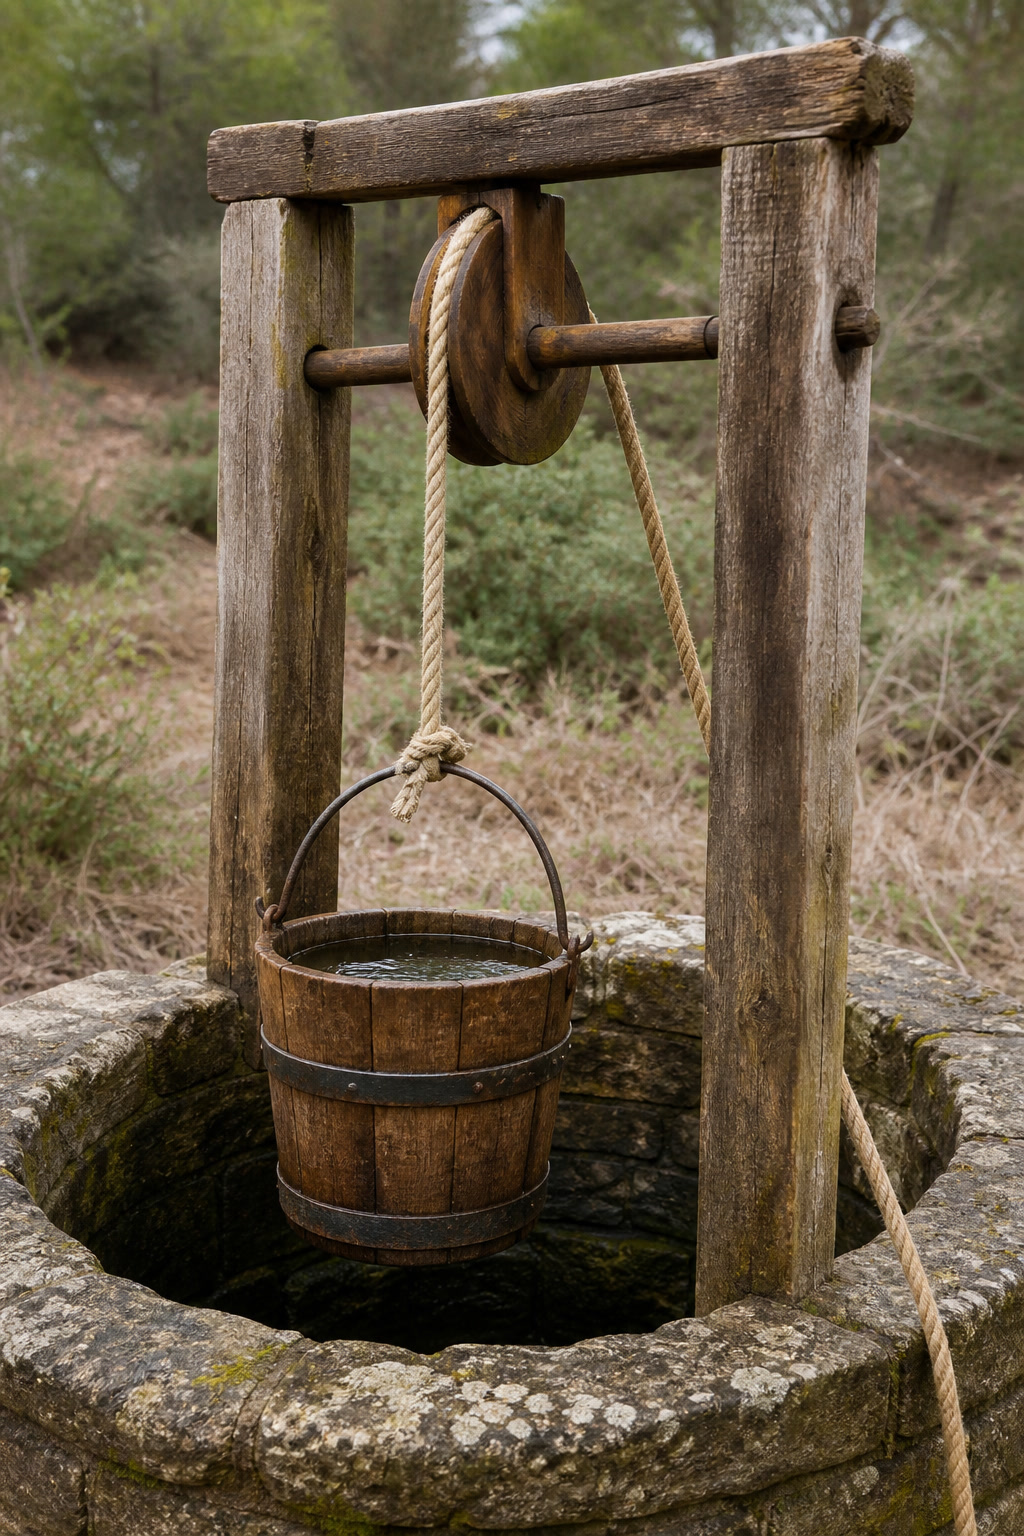
\includegraphics[width=0.34\linewidth]{images/book1/ai/g5-machines-pulley.jpg}

{\small 水井上的\omterm{def:g5:simple-machines:pulley}{滑轮}：绳子卧在绳槽里，向下的拉力变成了向上的提升。}
\end{omfigure}

\begin{example}[滑轮的应用]\label{ex:g5:simple-machines:pulleywork}
旗子沿旗杆向上升起，你的双手却轻松地
向\emph{下}拉：顶端是一个定\omterm{def:g5:simple-machines:pulley}{滑轮}，方向改变了，
用力大小不变，但向下拉时你自身的重量也能帮忙。建筑工人
使用的\omterm{def:g5:simple-machines:pulley}{滑轮}组把几个\omterm{def:g5:simple-machines:pulley}{滑轮}串在一起，使重物
悬挂在四股或六股绳子上：每股绳子只承担四分之一或六分之一
的重量，一名工人就能吊起一架钢琴。注意看这名工人，
不过要留意：绳子一米又一米地从他手中滑过，
而钢琴只是缓缓地向上升。
\end{example}

\section{斜面}

\begin{definition}[斜面]\label{def:g5:simple-machines:ramp}
\emph{斜面}\index{斜面}——就是斜坡——是一种
用来抬高重物、却不必直接竖直提起的斜坡。
坡面越平缓，推动重物沿它移动所需的推力就越小：
把木桶沿又长又缓的斜坡滚上去很容易；沿
又短又陡的斜坡则非常费力；竖直向上则不可能。
\end{definition}

\begin{method}[用橡皮筋测力计来感受]\label{met:g5:simple-machines:measure}
你去年用过的橡皮筋测力计能感受出这种差别：
\begin{enumerate}
  \item 把玩具小车放到木板上，并把橡皮筋挂在小车上；
  \item 把木板一端垫在一小摞书上，做成一个平缓的斜坡；用橡皮筋
        把小车慢慢拉上去，并记下橡皮筋伸长的长度；
  \item 把同一块木板垫得陡得多，一端搁在椅子座面上，然后
        再拉一次。
\end{enumerate}
陡坡上拉动时橡皮筋伸长得多：坡越陡，
所需的力越大。缓坡确实省力——测力计
也这样告诉你。
\end{method}

\begin{omfigure}
\begin{tikzpicture}[scale=0.8]
  \draw[thick] (0,0) -- (11.2,0);
  \draw[very thick, omDef] (0.3,0) -- (6.5,2.0);
  \draw[thick, fill=omMeth, fill opacity=0.4]
    (2.8,0.82) rectangle ++(0.8,0.55);
  \draw[-Stealth, thick, omThm] (3.75,1.35) -- (4.65,1.64);
  \node[above, font=\small, omThm] at (3.4,1.75) {小推力};
  \draw[very thick, omDef] (8.2,0) -- (10.2,2.0);
  \draw[thick, fill=omMeth, fill opacity=0.4]
    (8.75,0.5) rectangle ++(0.8,0.55);
  \draw[-Stealth, very thick, omThm] (9.75,1.25) -- (10.55,2.05);
  \node[above, font=\small, omThm] at (9.3,1.9) {大推力};
  \node[below, font=\small] at (3.4,-0.3)
    {通往同一高度的长而缓的斜坡};
  \node[below, font=\small] at (9.3,-0.3) {短陡坡};
\end{tikzpicture}

{\small 同一个箱子，要升高同样的高度：长而缓的斜坡要的是
小推力，但要沿很长的路推；陡而短的斜坡要的是大推力，
沿很短的路推。}
\end{omfigure}

\begin{example}[地形中的斜坡]\label{ex:g5:simple-machines:ramps}
轮椅坡道又长又缓，与短短的台阶并排而建——
这是有意为之。山路之所以盘旋曲折，是因为
不直接向山顶攀登，而是把一条长而缓的\omterm{def:g5:simple-machines:ramp}{斜面}
来回绕着山坡修。螺钉其实是伪装的\omterm{def:g5:simple-machines:ramp}{斜面}——
一个绕在杆上的\omterm{def:g5:simple-machines:ramp}{斜面}，所以螺丝刀每轻轻转一圈，
螺钉就悄悄地向里钻进一小步。
\end{example}

\section{黄金法则}

\begin{proposition}[机械的黄金法则]\label{prop:g5:simple-machines:golden}
任何\omterm{def:g5:simple-machines:machine}{简单机械}都不能白白得到好处：它省下的
力，必须在距离上补回来。省一半的力——拉动的绳子
长一倍，或走过的路程也翻一倍；省到十分之一的力——
路程就要长十倍。每一种机械都是如此，这笔交易分毫不差：
省力要用米来换。
\end{proposition}

\begin{example}[检验法则]\label{ex:g5:simple-machines:check}
动\omterm{def:g5:simple-machines:pulley}{滑轮}：手只用一半的力，
要把重物提起 \qty{1}{m}，就得拉进 \qty{2}{m} 的绳子——
两段绳子都要各缩短一米。撬棍：你这一端扫过一段
长长的弧线，而大石头几乎纹丝不动。\omterm{def:g5:simple-machines:ramp}{斜面}：箱子升到
同样的高度，但你是沿整个斜坡推上去的。每一笔省力
都分毫不差地付了代价。
\end{example}

\begin{remark}[为什么不能钻这条法则的空子]\label{rem:g5:simple-machines:whygolden}
藏在黄金法则背后的，正是\omterm{def:g5:everyday-energy:energy}{能量}一章里的老朋友：
把重物提升到一定高度，需要付出固定的\omterm{def:g5:everyday-energy:energy}{能量}，
无论怎样安排绳索和木板，都改变不了这个价格。
机械只是让你用更小的零钱来付，但要付更多次。小力
沿长路程移动，与大力沿短路程移动，
交出的\omterm{def:g5:everyday-energy:energy}{能量}相同。永动机之所以失败，
正是这个道理：账单总是那一笔。
\end{remark}

\section{练习}

\begin{exercise}[$\star$]\label{exo:g5:simple-machines:1}
说出三种经典的\omterm{def:g5:simple-machines:machine}{简单机械}，
并各举一个日常生活中会用到它们的地方。
\end{exercise}

\begin{exercise}[$\star$]\label{exo:g5:simple-machines:2}
定\omterm{def:g5:simple-machines:pulley}{滑轮}会改变你所用拉力的哪些方面？动\omterm{def:g5:simple-machines:pulley}{滑轮}
又会改变什么？
\end{exercise}

\begin{exercise}[$\star$]\label{exo:g5:simple-machines:3}
为什么往\emph{下}拉旗子来升旗，
比直接把同样重的东西向上提更舒服，
尽管用力的大小相同？
\end{exercise}

\begin{exercise}[$\star$]\label{exo:g5:simple-machines:4}
用一个动\omterm{def:g5:simple-machines:pulley}{滑轮}时，重物由两段绳子承担。
你的手承担\omterm{def:g4:weight-and-mass:weight}{重力}的几分之几？要把重物
提起 \qty{3}{m}，需要拉多长的绳子？
\end{exercise}

\begin{exercise}[$\star$]\label{exo:g5:simple-machines:5}
在\cref{met:g5:simple-machines:measure}中，哪一个\omterm{def:g5:simple-machines:ramp}{斜面}使橡皮筋
伸长得更多？较缓\omterm{def:g5:simple-machines:ramp}{斜面}较小的伸长
是用什么换来的？
\end{exercise}

\begin{exercise}[$\star$]\label{exo:g5:simple-machines:6}
为什么山路要盘旋，而不是沿着斜坡
笔直地向上？整条山路属于哪种\omterm{def:g5:simple-machines:machine}{简单机械}？
\end{exercise}

\begin{exercise}[$\star$]\label{exo:g5:simple-machines:7}
叙述机械的黄金法则。某台机械让你只用
十分之一的力去拉，它要你付出什么代价？
\end{exercise}

\begin{exercise}[$\star$]\label{exo:g5:simple-machines:8}
螺钉怎样是一种伪装的\omterm{def:g5:simple-machines:ramp}{斜面}？什么东西扮演
了那条长而缓道路的角色？
\end{exercise}

\begin{exercise}[$\star\star$]\label{exo:g5:simple-machines:9}
一个\omterm{def:g5:simple-machines:pulley}{滑轮}组用四段绳子悬挂一架钢琴。工人的手
拉的是钢琴\omterm{def:g4:weight-and-mass:weight}{重力}的几分之几？要把钢琴
提起 \qty{2}{m}，有多少米的绳子经过他们的
手？
\end{exercise}

\begin{exercise}[$\star\star$]\label{exo:g5:simple-machines:10}
一条装货斜坡长 \qty{6}{m}，升高 \qty{1}{m}，
把箱子推上去只需一个不大的推力。性急的搬运工
又修了一条只有 \qty{3}{m} 长、通往同一平台的新斜坡。用黄金法则，
比较新旧两种推力的大小，并说明为什么
“路程减半”并不划算。
\end{exercise}

\begin{exercise}[$\star\star$]\label{exo:g5:simple-machines:11}
一则广告推销一套\omterm{def:g5:simple-machines:pulley}{滑轮}组，宣称它“聪明得很：拉动一米绳子只需一半的力，
——重物却升高整整一米。
”。将这一宣称放到黄金法则和
\cref{rem:g5:simple-machines:whygolden}的\omterm{def:g5:everyday-energy:energy}{能量}账下检验：
任何轮与绳索的组合能否兑现它？
\end{exercise}
